\documentclass[journal,12pt,twocolumn]{IEEEtran}

\usepackage{setspace}
\usepackage{gensymb}

\singlespacing


\usepackage[cmex10]{amsmath}

\usepackage{amsthm}

\usepackage{mathrsfs}
\usepackage{txfonts}
\usepackage{stfloats}
\usepackage{bm}
\usepackage{cite}
\usepackage{cases}
\usepackage{subfig}

\usepackage{longtable}
\usepackage{multirow}

\usepackage{enumitem}
\usepackage{mathtools}
\usepackage{steinmetz}
\usepackage{tikz}
\usepackage{circuitikz}
\usepackage{verbatim}
\usepackage{tfrupee}
\usepackage[breaklinks=true]{hyperref}
\usepackage{graphicx}
\usepackage{tkz-euclide}

\usetikzlibrary{calc,math}
\usepackage{listings}
    \usepackage{color}                                            %%
    \usepackage{array}                                            %%
    \usepackage{longtable}                                        %%
    \usepackage{calc}                                             %%
    \usepackage{multirow}                                         %%
    \usepackage{hhline}                                           %%
    \usepackage{ifthen}                                           %%
    \usepackage{lscape}     
\usepackage{multicol}
\usepackage{chngcntr}

\DeclareMathOperator*{\Res}{Res}
\DeclareMathOperator{\taninv}{tan^{-1}}

\renewcommand\thesection{\arabic{section}}
\renewcommand\thesubsection{\thesection.\arabic{subsection}}
\renewcommand\thesubsubsection{\thesubsection.\arabic{subsubsection}}

\renewcommand\thesectiondis{\arabic{section}}
\renewcommand\thesubsectiondis{\thesectiondis.\arabic{subsection}}
\renewcommand\thesubsubsectiondis{\thesubsectiondis.\arabic{subsubsection}}


\hyphenation{op-tical net-works semi-conduc-tor}
\def\inputGnumericTable{}                                 %%

\lstset{
%language=C,
frame=single, 
breaklines=true,
columns=fullflexible
}
\begin{document}


\newtheorem{theorem}{Theorem}[section]
\newtheorem{problem}{Problem}
\newtheorem{proposition}{Proposition}[section]
\newtheorem{lemma}{Lemma}[section]
\newtheorem{corollary}[theorem]{Corollary}
\newtheorem{example}{Example}[section]
\newtheorem{definition}[problem]{Definition}

\newcommand{\BEQA}{\begin{eqnarray}}
\newcommand{\EEQA}{\end{eqnarray}}
\newcommand{\define}{\stackrel{\triangle}{=}}
\bibliographystyle{IEEEtran}
\providecommand{\mbf}{\mathbf}
\providecommand{\pr}[1]{\ensuremath{\Pr\left(#1\right)}}
\providecommand{\qfunc}[1]{\ensuremath{Q\left(#1\right)}}
\providecommand{\sbrak}[1]{\ensuremath{{}\left[#1\right]}}
\providecommand{\lsbrak}[1]{\ensuremath{{}\left[#1\right.}}
\providecommand{\rsbrak}[1]{\ensuremath{{}\left.#1\right]}}
\providecommand{\brak}[1]{\ensuremath{\left(#1\right)}}
\providecommand{\lbrak}[1]{\ensuremath{\left(#1\right.}}
\providecommand{\rbrak}[1]{\ensuremath{\left.#1\right)}}
\providecommand{\cbrak}[1]{\ensuremath{\left\{#1\right\}}}
\providecommand{\lcbrak}[1]{\ensuremath{\left\{#1\right.}}
\providecommand{\rcbrak}[1]{\ensuremath{\left.#1\right\}}}
\theoremstyle{remark}
\newtheorem{rem}{Remark}
\newcommand{\sgn}{\mathop{\mathrm{sgn}}}
\providecommand{\abs}[1]{\left\vert#1\right\vert}
\providecommand{\res}[1]{\Res\displaylimits_{#1}} 
\providecommand{\norm}[1]{\left\lVert#1\right\rVert}
%\providecommand{\norm}[1]{\lVert#1\rVert}
\providecommand{\mtx}[1]{\mathbf{#1}}
\providecommand{\mean}[1]{E\left[ #1 \right]}
\providecommand{\fourier}{\overset{\mathcal{F}}{ \rightleftharpoons}}
%\providecommand{\hilbert}{\overset{\mathcal{H}}{ \rightleftharpoons}}
\providecommand{\system}{\overset{\mathcal{H}}{ \longleftrightarrow}}
	%\newcommand{\solution}[2]{\textbf{Solution:}{#1}}
\newcommand{\solution}{\noindent \textbf{Solution: }}
\newcommand{\cosec}{\,\text{cosec}\,}
\providecommand{\dec}[2]{\ensuremath{\overset{#1}{\underset{#2}{\gtrless}}}}
\newcommand{\myvec}[1]{\ensuremath{\begin{pmatrix}#1\end{pmatrix}}}
\newcommand{\mydet}[1]{\ensuremath{\begin{vmatrix}#1\end{vmatrix}}}
\numberwithin{equation}{subsection}
\makeatletter
\@addtoreset{figure}{problem}
\makeatother
\let\StandardTheFigure\thefigure
\let\vec\mathbf
\renewcommand{\thefigure}{\theproblem}
\def\putbox#1#2#3{\makebox[0in][l]{\makebox[#1][l]{}\raisebox{\baselineskip}[0in][0in]{\raisebox{#2}[0in][0in]{#3}}}}
     \def\rightbox#1{\makebox[0in][r]{#1}}
     \def\centbox#1{\makebox[0in]{#1}}
     \def\topbox#1{\raisebox{-\baselineskip}[0in][0in]{#1}}
     \def\midbox#1{\raisebox{-0.5\baselineskip}[0in][0in]{#1}}
\vspace{3cm}
\title{Assignment 1}
\author{Pulkit Saxena}
\maketitle
\newpage
\bigskip
\renewcommand{\thefigure}{\theenumi}
\renewcommand{\thetable}{\theenumi}

%
Download all python codes from 
\begin{lstlisting}
https://github.com/pulkitsaxena92/IITH-EE5609/tree/master/assignment%201/code
\end{lstlisting}
%
and latex-tikz codes from 
%
\begin{lstlisting}
https://github.com/pulkitsaxena92/IITH-EE5609/tree/master/assignment%201
\end{lstlisting}
\section{Question No. 42}
Find the equation of lines through the point \myvec{3\\2}  which make an angle of 45$^{\circ}$ to the line

\begin{align}
\myvec{1 & -2}\vec{x} = 3 
\end{align}
\section{Explanation}
\subsection{Assumption}
Let $m_2$ be the slope of the other Line
\subsection{Formulae Used}
1) Equation of Line Passing through \myvec{3\\2} with a normal Vector is given by
\begin{align}
    n^T(X-A)=0 
\end{align}
where A is the point satisfying the Equation.
\\2) Inner Product of two vectors is given by the formulae
\begin{align}
 \cos \theta &= \frac{\vec{n_1}^T\vec{n_2}}{\norm{\vec{n_1}}\norm{\vec{n_2}}}\\   
\end{align}
where is the angle between two lines
\\3)Normal Vector For Second Line is given by
\begin{align}
n_2=\myvec{-m_2\\1}
\end{align}
Where $m_2$ is the slope of second line
\subsection{Solution}
On comparing $\myvec{1 & -2}\vec{x} = 3$ with Formulae 1  we get 
\begin{align}
    n_1^T=\myvec{1 & -2}
\end{align}
\begin{align}
  n_2=\myvec{-m_2\\1}  
\end{align}
\begin{align}
    \theta=45^\circ
    \implies \cos 45\degree &=\frac{1}{\sqrt{2}}\\ 
\end{align}
Substuting $n_1^T$ $n_2$ and $\theta$ in Formulae 2  we get
\begin{align}
    \frac{1}{\sqrt{2}}=\frac{\myvec{1 & -2}\times\myvec{-m_2\\1}}{\sqrt{5}\times\sqrt{m_2^2+1}}
\end{align}
\begin{align}
    3m_2^2-4m_2-3=0
    \implies m_2=3,-\frac{1}{3}
\end{align}
\subsubsection{Case 1}
Equations of Line with Slope $m_2=3$ and passing through point $\myvec{3\\2}$ is given as
\begin{align}
  n^T(X-A)=0   
\end{align}
Substuting Values we get
\begin{align}
 \myvec{-3 & 1}\myvec{X-\myvec{3\\2}}=0\\
 \myvec{-3 & 1}x=-7
\end{align}
\subsubsection{Case 2}
Equations of Line with Slope $m_2=-\frac{1}{3}$ and passing through point $\myvec{3\\2}$ is given as
\begin{align}
  n^T(X-A)=0   
\end{align}
Substuting Values we get
\begin{align}
 \myvec{\frac{1}{3} & 1}\myvec{X-\myvec{3\\2}}=0\\
 \myvec{\frac{1}{3} & 1}x=3
\end{align}
\subsection{Answers}
the equation of lines through the point \myvec{3\\2}  which make an angle of 45$^{\circ}$ to the line

\begin{align}
\myvec{1 & -2}\vec{x} = 3 
\end{align}
are
\begin{align}
   \myvec{-3 & 1}x=-7\\ 
   \myvec{\frac{1}{3} & 1}x=3
\end{align}
The Figure below shows the plot of all three lines
\begin{figure}[!ht]
\centering
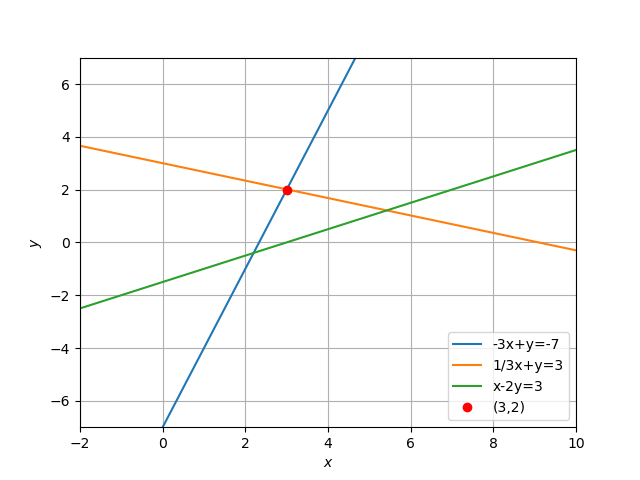
\includegraphics[width=\columnwidth]{Edit_plot.png}
\caption{Plotting these Equation}
\end{figure}
\end{document}
